% !TEX root= ../main.tex
\section{Results in Kernel Theory}
\label{sec:Results in Kernel Theory}
There exists many results in Kernel Theory regarding finitary\footnote{In a finitary graph, every vertex has a finite number of out-neighbors; the graph has finite branching.} digraphs, one of them being the Richardson's Theorem:\\

\begin{theorem}
  \cite{am-richardson} If D is a finitary digraph without odd cycles, then D has a kernel.
\end{theorem}
It seems natural that graphs with no odd cycles can guarantee us a kernels, but why does the graph have to be finitary?
Can there be an acyclic graph with no kernels, thus modelling a paradoxical discourse?
Until now, our paradoxes have always been -- directly or indirectly -- referring back to itself and thus causing the conflict, but the following construction will be an exception from that trend.

The \textbf{Yablo Graph} \cite{analysis-yablo} is an example of an acyclic graph with no kernel. It is constructed with an infinite set of vertices $\{ x_i | i \in \mathbb{N} \}$ and a set of edges $N$ such that $\langle x_i, x_j \rangle \in N$ iff $i < j$.
\[
  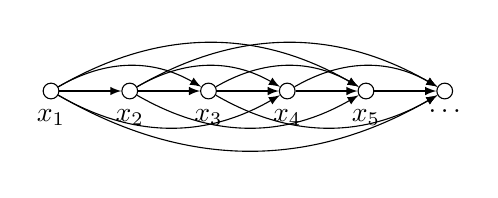
\begin{tikzpicture}
    [
    point/.style={circle,draw,inner sep=0pt,minimum size=2mm},
    collection/.style={thick,rectangle,draw,inner sep=0pt,minimum height=14mm, minimum width= 9mm}
    ]
    \node (1) at (0,1) [point,label=below:$x_1$] {};
    \node (2) at (1,1) [point,label=below:$x_2$] {};
    \node (3) at (2,1) [point,label=below:$x_3$] {};
    \node (4) at (3,1) [point,label=below:$x_4$] {};
    \node (5) at (4,1) [point,label=below:$x_5$] {};
    \node (6) at (5,1) [point,label=below:$\dots$] {};
    \draw [-latex] (1) to (2);
    \draw [-latex] (2) to (3);
    \draw [-latex] (3) to (4);
    \draw [-latex] (4) to (5);
    \draw [-latex] (5) to (6);
    \draw [-latex, bend left] (1) to (3);
    \draw [-latex, bend left] (2) to (4);
    \draw [-latex, bend left] (3) to (5);
    \draw [-latex, bend left] (4) to (6);
    \draw [-latex, bend right] (1) to (4);
    \draw [-latex, bend right] (2) to (5);
    \draw [-latex, bend right] (3) to (6);
    \draw [-latex, bend left] (1) to (5);
    \draw [-latex, bend left] (2) to (6);
    \draw [-latex, bend right] (1) to (6);
  \end{tikzpicture}
\]

Since there exist no two numbers $x,y \in \mathbb{N}$ such that $x < y$ and $y < x$, we get that the Yablo graph indeed is acyclic.
Furthermore, since any natural number has infinitely many numbers strictly larger than it, we get that all the vertices are infinitely branching, making the Yablo graph infinitary (not finitary).
We will later show that this graph is indeed without a kernel, but for now we will take Yablo's word \cite{analysis-yablo} for it.
